\documentclass{article}
%\usepackage{tex4ht}
\usepackage{amsmath}
\usepackage{amsfonts}
\usepackage{amssymb}
\usepackage{amsthm}
\usepackage{graphicx}
\usepackage{color}
\usepackage{float}
\usepackage{dsfont}
\usepackage{hyperref}
\setlength{\parskip}{0.5\baselineskip}
\author{Zhuo Liu (0983311)}
\title{Homework 2 for Database Systems}
\date{May 5, 2014}

\definecolor{lightgray}{gray}{0.5}


\begin{document}
\maketitle

\section{Section 1}

The size of the table is $n$ records (rows) and $l$ features (columns).

%%% -----------------------------------------------------------------------------------------------------------------------------------------------------------------------------------
\goodbreak

\subsection{Multilevel Index}

Suppose there are $k$ levels for index and each block can hold $m_{1}$ records and $m_{2}$ index. If without considering blocks and disk access, the $O()$ analysis is as follows:

Insert:
since there are $k$ levels, number of index in root level will be $\frac{n}{m_{1}m_{2}^{k-1}}$. We can use binary search to find proper position in root level, so the cost on this level will be $O(\log{n}-\log{m_{1}}-(k-1)\log{m_{2}})$. Then we can do binary search for level $2$ to level $k$, and for each level we only need to do binary search in $m_{2}$ index and $m_{1}$ in final block, so the total cost for searching will be $(k-1)*O(\log{m_{2}})+O(\log{m_{1}})$. Therefore, to find the final position, the total cost will be:
\begin{equation*}
O(\log{n}-\log{m_{1}}-(k-1)\log{m_{2}}) + (k-1)O(\log{m_{2}}) + O(\log{m_{1}})= O(\log{n}),
\end{equation*}
and there should be a $O(1)$ cost for insertion into this position, so the total cost will be $O(\log{n}+1)$.

Delete:
similar to insert, the cost will be $O(\log{n}+1)$, $O(1)$ represent the cost for deletion on the position found.

Search:
the cost will be $O(\log{n})$ as analyzed above.

If considering blocks and disk access, besides the cost of searching in each block, we also need to consider the number of blocks accessed (Or whose data is read into RAM). The number of blocks accessed will be equal to the number of levels, so for all the cost above, we need to add one more term: $c*O(k)$, where $c$ is the ratio between the cost in disk and RAM. Next table shows the conclusion for multilevel index:

 \begin{tabular}{|c|c|c|}
  \hline
  Multilevel Index & Without block access    & With block access \\ \hline
  Insert           & $O(\log{n}+1)$ & $O(\log{n}+1)+c*O(k)$  \\ \hline
  Delete           & $O(\log{n}+1)$ & $O(\log{n}+1)+c*O(k)$ \\ \hline
  Search           & $O(\log{n})$   & $O(\log{n})+c*O(k)$ \\ \hline
 \end{tabular}

%%% -----------------------------------------------------------------------------------------------------------------------------------------------------------------------------------
\goodbreak

\subsection{Hashing}

Suppose hash table is big enough and hash function is good enough, so in each bucket, there are only $O(1)$ records.

If without considering blocks and disk access: for insertion, deletion and search, we need first use hash function to find proper bucket, then go through the records in this bucket to find proper position to insert or find desired record. Since there are only $O(1)$ records in each bucket, so the cost will be only $O(1)$.

If we consider the block access, then we need to traverse all the records in one bucket. Suppose one block can hold $m_{3}$ addresses for records, then we need to access $O(\frac{1}{m_{3}})$ blocks. Suppose $c$ is the ratio between the cost in disk and RAM, then we need to add one more term $c*O(\frac{1}{m_{3}})$ for result when not considering disk access. The following table shows the result:

 \begin{tabular}{|c|c|c|}
  \hline
  Hashing          & Without block access & With block access \\ \hline
  Insert           & $O(1)$               & $O(1)+c*O(\frac{1}{m_{3}})$  \\ \hline
  Delete           & $O(1)$               & $O(1)+c*O(\frac{1}{m_{3}})$ \\ \hline
  Search           & $O(1)$               & $O(1)+c*O(\frac{1}{m_{3}})$ \\ \hline
 \end{tabular}

%%% -----------------------------------------------------------------------------------------------------------------------------------------------------------------------------------
\goodbreak

\subsection{B-Trees}

Suppose each block have space for $r$ search key values and $r+1$ pointers, then the depth of the B-tree will be of $O(\log_{r}{n})$. Without considering the access to blocks, on each level, we can do binary search, so the total cost for search is $O(\log_{r}{n}*\log_{2}{r})$. To delete or insert record, we need to do these operations on proper position, suppose the cost is $O(1)$, and maybe need to update one block for each level of B-tree, so the total costs for deletion and insertion will be $2*O(\log_{r}{n}*\log_{2}{r})+O(1)$.

If considering block access, the number of blocks accessed for search will be $O(\log_{r}{n})$ and for insertion and deletion will be $2*O(\log_{r}{n})$, so we need to add $c$ times these two number when considering block access, if $c$ is the ratio between the cost in disk and RAM. The following table shows the result:

 \begin{tabular}{|c|c|c|}
  \hline
  B-Trees          & Without block access                & With block access \\ \hline
  Insert           & $2*O(\log_{r}{n}*\log_{2}{r})+O(1)$ & $2*(O(\log_{r}{n}*\log_{2}{r}+c*O(\log_{r}{n}))+O(1)$  \\ \hline
  Delete           & $2*O(\log_{r}{n}*\log_{2}{r})+O(1)$ & $2*(O(\log_{r}{n}*\log_{2}{r}+c*O(\log_{r}{n}))+O(1)$ \\ \hline
  Search           & $O(\log_{r}{n}*\log_{2}{r})$        & $O(\log_{r}{n}*\log_{2}{r})+c*O(\log_{r}{n})$ \\ \hline
 \end{tabular}

%%% -----------------------------------------------------------------------------------------------------------------------------------------------------------------------------------
\goodbreak

\subsection{Ordered Tables}

Suppose each block can hold $m_{4}$ values in a column. Without considering block access, for search, we need to first find the position of the PKs, this cost will be $O(\log{n})$. Since we know the location of the record, then we need to find the its element in each column, this cost will be $l*O(1)$, so the total cost for search is $O(\log{n}+l)$, and the cost for insertion and deletion will be $O(\log{n}+l)+l*O(1)$, where the second $l*O(1)$ is the cost for insertion or deletion in each column.

When considering block access, to locate the value of the desired record in each column, $O(\frac{n}{m_{4}})$ blocks will be accessed. Therefore, we need to add another $l*O(\frac{n}{m_{3}})$ for above costs. The following table shows the result:

 \begin{tabular}{|c|c|c|}
  \hline
  Ordered Tables   & Without block access                & With block access \\ \hline
  Insert           & $O(\log{n}+l)+l*O(1)$ & $O(\log{n}+l)+l*O(1)+l*O(\frac{n}{m_{4}})$  \\ \hline
  Delete           & $O(\log{n}+l)+l*O(1)$ & $O(\log{n}+l)+l*O(1)+l*O(\frac{n}{m_{4}})$ \\ \hline
  Search           & $O(\log{n}+l)$        & $O(\log{n}+l)+l*O(\frac{n}{m_{4}})$ \\ \hline
 \end{tabular}


%%% -----------------------------------------------------------------------------------------------------------------------------------------------------------------------------------
\goodbreak

\section{Section 2}

Suppose there are two tables $T_{1}$ and $T_{2}$, with sizes $m$ and $n$. Consider the join operation on these two tables: $T_{1}(X,Y)\Join T_{2}(Y,Z)$, where $X,Y,Z$ are attributes in $T_{1}$ and $T_{2}$, correspondingly. Suppose we need $B(m)\sim O(m)$ and $B(n)\sim O(n)$ blocks to store table $T_{1}$ and $T_{2}$. Assume when there is seek disk access speed is 1000X slower than RAM random access, but if doing sequential access assume disk is just 10X slower.

\subsection{Nested-Loop Join}

Since this algorithm requires to analyze all the rows in $T_{1}$ and $T_{2}$, so the total number of comparison is $mn$, so the cost is of $O(mn)$. Moreover, the total number of blocks read is $B(m)B(n)$, and it is sequential access, so the time is approximately $10B(m)B(n)$.

%%% -----------------------------------------------------------------------------------------------------------------------------------------------------------------------------------
\goodbreak

\subsection{Sort-Based Join}

If attributes $Y$ is sorted, then similar to the idea of merge sort, the number of comparison is of $O(m+n)$. As a result, the number of blocks accessed will be $B(m)+B(n)$, and it is sequential access, so the time for r/w is $10(B(m)+B(n))$. However, at most of the time, $Y$ is unsorted, we need to use external merge sort algorithm to sort table $T_{1}$ and $T_{2}$ based on $Y$. Therefore, the cost for sorting is $O(\log{m}+\log{n})$, and the number of blocks read and write will be of $4(B(m)+B(n))$, which is sequential access, and we need to random access $B(m)+B(n)$ blocks to merge two tables. In conclusion, the time for r/w is of $1040(B(m)+B(n))$.

%%% -----------------------------------------------------------------------------------------------------------------------------------------------------------------------------------
\goodbreak

\subsection{Hash-Join}

We first create hash table for attributes $Y$ in the table with less records, suppose $m<n$, so $T_{1}$. Then scan $T_{2}$ and find the relevant rows from $T_{1}$ by looking in the hash table. Suppose the hash table is large enough and hash funcion is well-chosen, then the number of records in each buckets will be of $O(1)$, so the cost will be of $O(m+n)$. In order to build hash table, we need to read all the blocks, the number is $3(B(m)+B(n))$ which is sequential access, and write hash buckets, the number is $O(m+n)$ which is random access. Then we need to ``probe'' hash table, which is sequential access to $O(m+n)$ buckets. Therefore, the time for r/w is about $30(B(m)+B(n))+1010*O(m+n)$.

%%% -----------------------------------------------------------------------------------------------------------------------------------------------------------------------------------
\goodbreak

\subsection{Join by Using Index}

If there is index on attributes $Y$ in both $T_{1}$ and $T_{2}$, and suppose the index is sorted (i.e. B-trees), then we can simply scan the leaves of the two B-trees from left to right to decide which pairs of records can be joined, the idea is very similar to merge in merge sort, the cost will be of $O(m+n)$. However, since index are stored in blocks different than the original relations, suppose the number of blocks to store index are $B(\hat{m})$ and $B(\hat{n})$, which are much smaller than $B(m)$ and $B(n)$, then we need to read these blocks (sequential access). In addition, if we find one pair of records can be joined, we need to access corresponding blocks and write it (randomly access). If there are $k$ records for the result $T_{1}(X,Y)\Join T_{2}(Y,Z)$, then the total cost for r/w is $10(B(\hat{m})+B(\hat{n}))+2000k$.

%%% -----------------------------------------------------------------------------------------------------------------------------------------------------------------------------------
\goodbreak

\section{Section 3}

\subsection{2PL and Timestamping}

The differnces for the perfomance of 2PL and timestamping are:

\noindent (1) Storage utilization: For 2PL, space in the lock table is proportional to the number of database elements locked. For timestamping, space is needed for read- and write-times with every database element, whether or not it is currently accessed. Thus, the amounts of space used by each approach is approximately proportional to the sum over all active transactions of the number of database elements the transaction accesses. But timestamping may use slight more space.

\noindent (2) Locking will frequently delay transactions as they wait for locks, and if concurrent transactions frequently read and write elements in common, then rollbacks will be frequent in a timestamp scheduler, introducing even more delay than a locking system. Therefore, timestamping is superior in situations where either most transactions are read-only, or it is rare that concurrent transactions will try to read and write the same element. In high-conflict situations, locking performs better.

\noindent (3) Delay, Rollback and Overhead: 2PL delays transactions but avoids rollbacks, even when interaction is high. Timestamps does not delay transactions, but can cause them to rollback, which is a more serious form of delay and also wastes resources. Therefore, when interference if low, timestamp is better because it generally has lower overhead than 2PL. But if interference if high, 2PL is better because rollbacks waste much more resources.

%%% -----------------------------------------------------------------------------------------------------------------------------------------------------------------------------------
\goodbreak

\subsection{Queued Transaction Process}

For real DBMS, to handle queues of waiting transactions, there will be two queues: request queue and reply queue. The server program starts a transaction and dequeues the next request from the request queue. The server then does the work that the request is asking for, enqueues the reply to the reply queue, and commits, see Figure 1.

\begin{figure}[htp]
\centering
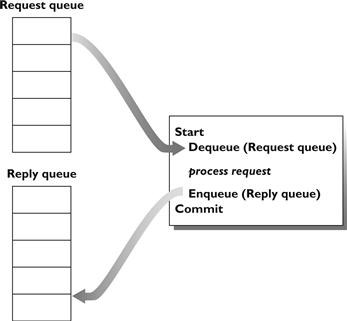
\includegraphics[width=8.4cm]{queued_TP.jpg}
\caption{\textit{Managing a Queued Request within a Transaction. The request is dequeued and the reply enqueued within a transaction. If the transaction aborts, the request is not lost.}}
\end{figure}


Since these queues are transactional resources, if the transaction aborts, the dequeue operation that receives the request is undone, thereby returning the input request to the request queue. If the abort happens at the very end, then the enqueue operation to the reply queue also is undone, thereby wiping out the reply from the reply queue. Therefore, whenever the client checks the queues, either the request is in the request queue, the reply is in the reply queue, or the request can¡¯t be checked because it is currently being processed. In any case, there¡¯s never any ambiguity as to the request¡¯s state. It either has not yet been processed, is in the midst of being processed, or has been completed.

%%% -----------------------------------------------------------------------------------------------------------------------------------------------------------------------------------
\goodbreak

\subsection{Graphs for 2PL and Timestamping}

Suppose there are $N$ transactions $T_{1}...T_{N}$, executed by $M$ threads where $M<<N$. 

If we fix $M$ and increase $N$, then when $N$ is small, interference if low, timestamp is better than 2PL. But when $N$ is large, interference if high, timestamp performs worse than 2PL. Figure 2 shows the graph for number of transactions/second as $N$ increases when $M$ is fixed.

\begin{figure}[htp]
\centering
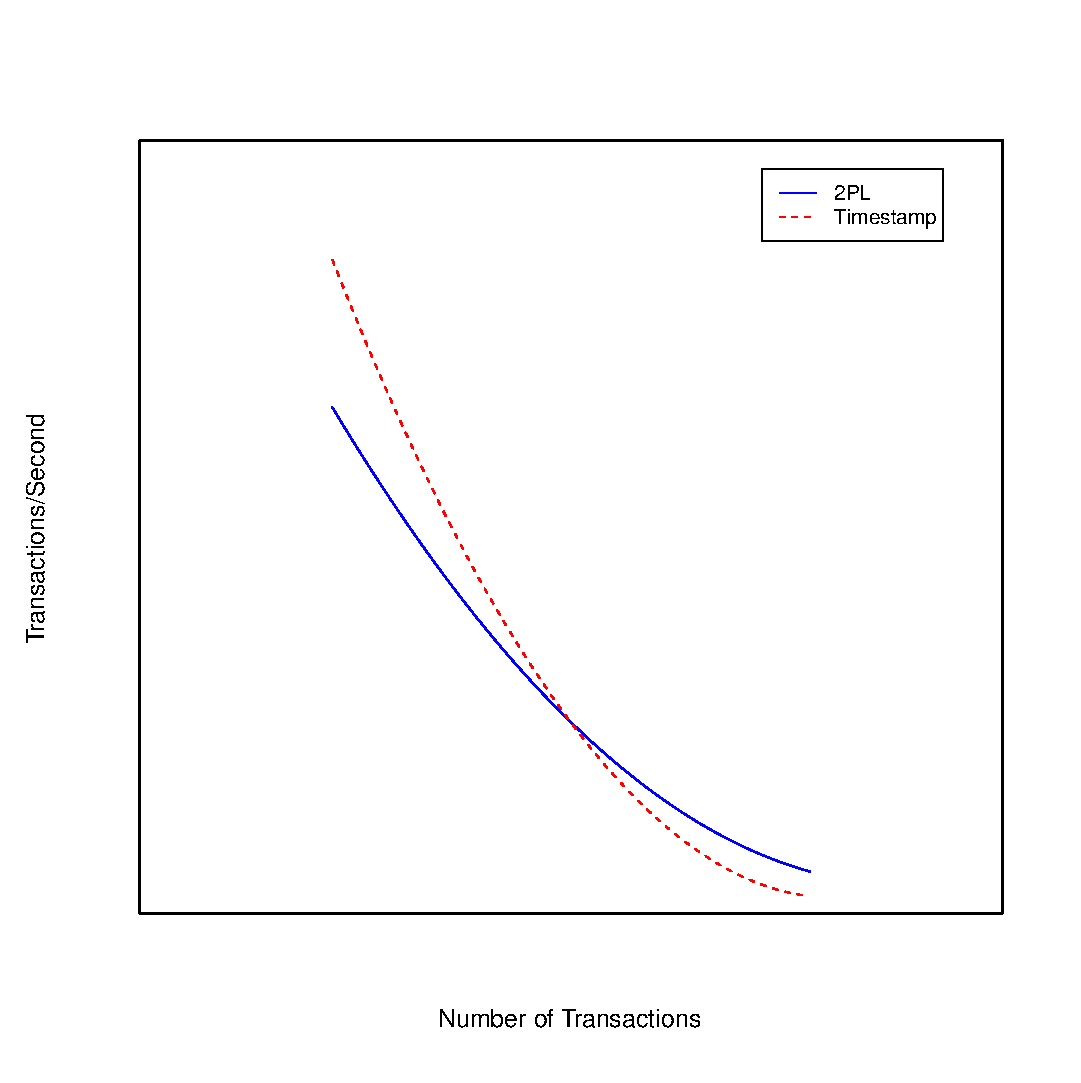
\includegraphics[width=9cm]{2pl_vs_ts_1.eps}
\caption{\textit{Graph for number of transactions/second as $N$ increases when $M$ is fixed.}}
\end{figure}

If we fix $N$ but increase $M$, then more threads will process more transactions in unit time. However, more threads also indicates more concurrent transactions, so more transactions will be delayed or rollback, therefore, the grapg for this case is shown in Figure 3.

\begin{figure}[htp]
\centering
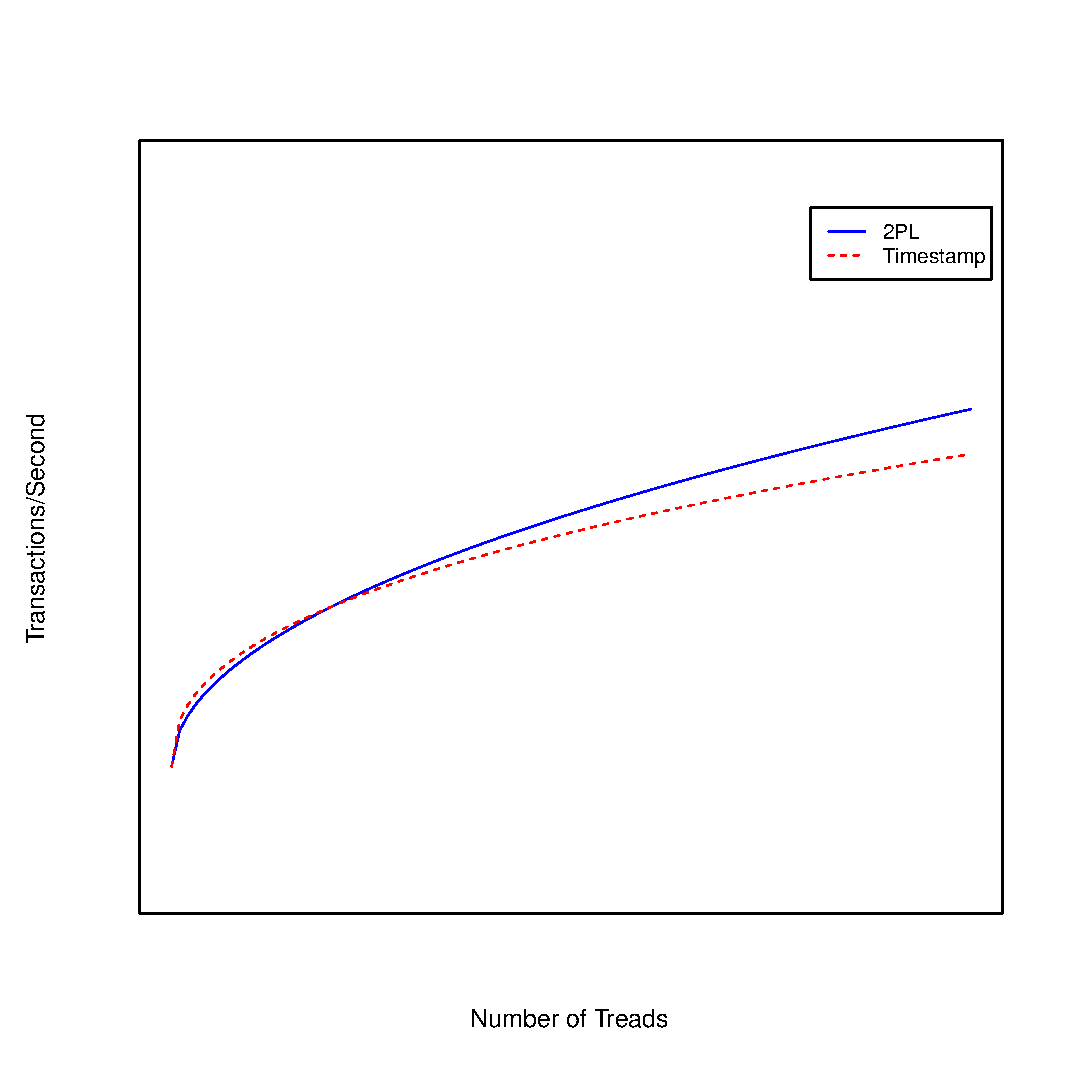
\includegraphics[width=9cm]{2pl_vs_ts_2.eps}
\caption{\textit{Graph for number of transactions/second as $M$ increases when $N$ is fixed.}}
\end{figure}

%%% -----------------------------------------------------------------------------------------------------------------------------------------------------------------------------------
\goodbreak

\section{Section 4}

For SSD, there are some charateristics:

\noindent (1) Uniform random access speed, and accessing data is almost proportional to the amount of data accesse. (Only requires data transfer time, seek time and rational latency can be ignored)

\noindent (2) Writing is expensive. Writing can only be done to an empty space, it is costly to erase data – Erasing data can only be done in erase units, typically $>=$ 128 kbytes. Because of this SSDs do not generally store data sequentially.

\noindent (3) Assymetric speed (reading is twice as fast as writing).


Therefore, SSD is much faster than HDD for random access, but has no significant difference on sequential access.

As a result, for the operation ``insert'', ``delete'', ``select...where... (search)'', since we need more random access to data (find proper position), so SSD will perform much better than HDD. However, for operation ``select *'', it mainly requires sequential access to data, so the perfomances on SSD and HDD have no significant difference.

For nest-loop join, only sequential access is needed, so SSD and HDD perfomance similarly. But for sort-based join, hash-join and index-join, both sequential and random accesses are required, so SSD will be much faster than HDD.

%%% -----------------------------------------------------------------------------------------------------------------------------------------------------------------------------------
\goodbreak

\newpage

\begin{thebibliography}{9}

\bibitem{molina09}
  Hector Garcia-Molina, Jeffrey D. Ullman, Jennifer Widom,
  \emph{Database Systems - The Complete Book}.
  Pearson Prentice Hall, Upper Saddle River, New Jersey,
  2nd Edition,
  2009.
  
\bibitem{bernstein09}
   Philip A. Bernstein, Eric Newcomer, 
   \emph{Principles of Transaction Processing}.
   Morgan Kaufmann, 2nd Edition, 2009
   
\bibitem{}
   Glen Berseth,
   \emph{SSDs vs HDDs for DBMS}.
   York University, Toronto
   
   \url{http://www.cse.yorku.ca/~jarek/courses/6421/F12/presentations/SSD_Presentation.pdf}
   
\bibitem{}
   Ki Yeul Lee,
   \emph{Will the use of SSD increase the speed of DBMS}?
   
   \url{http://www.cubrid.org/blog/dev-platform/will-the-use-of-ssd-increase-the-speed-of-dbms/}

\end{thebibliography}

\end{document}


